Le pratiche agili suggeriscono l'utilizzo di \textit{user story} per la descrizione del comportamento del sistema.

Una \textit{user story} � una frase composta utilizzando il linguaggio naturale, che descrive una particolare caratteristica del sistema in oggetto.

La struttura della frase da comporre � prefissata e si compone di tre entit� fondamentali: \textit{chi}, \textit{cosa} e \textit{perch�}. Attraverso questi tre concetti � possibile descrivere il comportamento atteso da un attore nel sistema (umano o software) che esegue una determinata azione con al fine di ottenere un risultato.

Le frasi devono essere concise, in modo da rappresentare una funzionalit� ben definita del sistema.

stime delle storie

La \textit{user story} � tipicamente scritta su un biglietto adesivo, e incollata ad una lavagna che riporta l'insieme dei requisiti del sistema.

La creazione delle storie, tipicamente avviene da parte del cliente, durante questo processo l'\textit{owner} lo guida nella stesura attraverso domande specifiche, in modo da aiutarlo a formalizzare le funzionalit� necessarie.

Ogni storia rappresenta una funzionalit� ben precisa sviluppabile tipicamente in un periodo che va da alcuni giorni a un paio di settimane.

Scrivere aiuta il cliente a concretizzare la sua idea di come deve funzionare il sistema, perch� spesso i requisiti sono fumosi.


Abbiamo scelto di usare le \textit{user story} perch� sono un metodo molto efficace per descrivere i requisiti del sistema utilizzando un linguaggio informale. Se cambiano le esigenze � molto facile sostituire le user story, al tempo stesso tutti i requisiti importanti sono sott'occhio.

L'utilizzo delle user story si lega a quello del TDD, infatti il successo nella realizzazione di ogni storia va confermato con test a corredo del software che implementa tale requisito.

%TODO inserire una immagine di una lavagna con user story oppure di un postit con una storia di esempio

\begin{figure}[h]
\centering
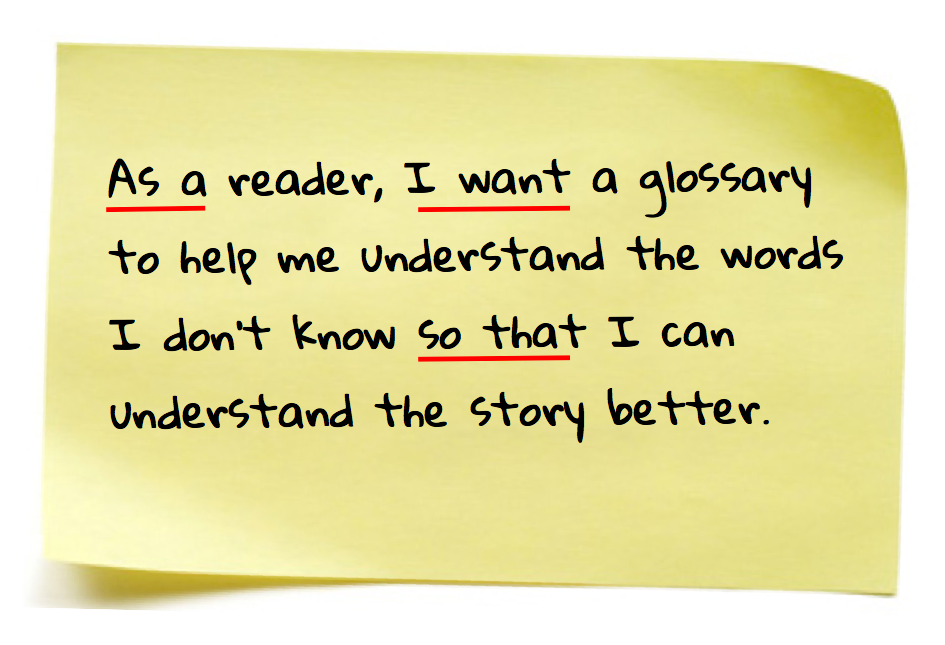
\includegraphics[width=0.7\linewidth]{./img/user-story}
\caption[Un esempio di \textit{user story}]{Un esempio di \textit{user story}}
\label{fig:user-story}
\end{figure}


%In software development and product management, a user story is one or more sentences in the everyday or business language of the end user or user of a system that captures what a user does or needs to do as part of his or her job function. User stories are used with agile software development methodologies as the basis for defining the functions a business system must provide, and to facilitate requirements management. It captures the 'who', 'what' and 'why' of a requirement in a simple, concise way, often limited in detail by what can be hand-written on a small paper notecard. User stories are written by or for the business user as that user's primary way to influence the functionality of the system being developed. User stories may also be written by developers to express non-functional requirements (security, performance, quality, etc.),[1] though primarily it is the task of a product manager to ensure user stories are captured.
%User stories are a quick way of handling customer requirements without having to create formalized requirement documents and without performing administrative tasks related to maintaining them. The intention of the user story is to be able to respond faster and with less overhead to rapidly changing real-world requirements.
%A user story is an informal statement of the requirement as long as the correspondence of acceptance testing procedures is lacking. Before a user story is to be implemented, an appropriate acceptance procedure must be written by the customer to ensure by testing or otherwise whether the goals of the user story have been fulfilled. Some formalization finally happens when the developer accepts the user story and the acceptance procedure as a work specific order.

%Creating user stories
%When the time comes for creating user stories, one of the developers (or the product owner in Scrum (development) ) gets together with a customer representative. The customer has the responsibility for formulating the user stories. The developer may use a series of questions to get the customer going, such as asking about the desirability of some particular functionality, but must take care not to dominate the idea-creation process.
%As the customer conceives the user stories, they are written down by the customer on a note card (e.g. 3x5 inches or 8x13 cm) with a name and a description which the customer has formulated. If the developer and customer find a user story deficient in some way (too large, complicated, imprecise), it is rewritten until it is satisfactory - often using the INVEST guidelines from the Scrum project-management framework. However, Extreme Programming (XP) emphasizes that user stories are not to be definite once they have been written down. Requirements tend to change during the development period, which the process handles by not carving them in stone.

%Benefits
%XP and other agile methodologies favor face-to-face communication over comprehensive documentation and quick adaptation to change instead of fixation on the problem. User stories achieve this by:
%Being very short. They represent small chunks of business value that can be implemented in a period of days to weeks.
%Allowing developer and the client representative to discuss requirements throughout the project lifetime.
%Needing very little maintenance.
%Only being considered at the time of use.
%Maintaining a close customer contact.
%Allowing projects to be broken into small increments.
%Being suited to projects where the requirements are volatile or poorly understood. Iterations of discovery drive the refinement process.
%Making it easier to estimate development effort.
%Require close customer contact throughout the project so that the most valued parts of the software get implemented.